\documentclass{beamer}
\usepackage[utf8]{inputenc}
\usepackage{graphicx, epsfig}
\usepackage{amsmath,mathrsfs,amsfonts,amssymb}
\usepackage{floatflt}
\usepackage{epic,ecltree}
\usepackage{mathtext}
\usepackage{fancybox}
\usepackage{fancyhdr}
\usepackage{multirow}
\usepackage{enumerate}
\usepackage{epstopdf}
\usepackage{multicol}
\usepackage{algorithm}
\usepackage[noend]{algorithmic}
\usepackage{tikz}
\usepackage{blindtext}
\usetheme{default}%{Singapore}%{Warsaw}%{Warsaw}%{Darmstadt}
\usecolortheme{default}

\setbeamerfont{title}{size=\Huge}
\setbeamertemplate{footline}[page number]{}

\setbeamertemplate{section in toc}[sections numbered]


\makeatletter
\newcommand\HUGE{\@setfontsize\Huge{35}{40}}
\makeatother    

\setbeamerfont{title}{size=\HUGE}
\beamertemplatenavigationsymbolsempty

% latin bold lower
\newcommand{\ba}{\mathbf{a}} 
\newcommand{\bc}{\mathbf{c}} 
\newcommand{\be}{\mathbf{e}} 
\newcommand{\bh}{\mathbf{h}} 
\newcommand{\bp}{\mathbf{p}} 
\newcommand{\bt}{\mathbf{t}} 
\newcommand{\bs}{\mathbf{s}} 
\newcommand{\bu}{\mathbf{u}} 
\newcommand{\bv}{\mathbf{v}} 
\newcommand{\bw}{\mathbf{w}} 
\newcommand{\bx}{\mathbf{x}} 
\newcommand{\by}{\mathbf{y}} 
\newcommand{\bz}{\mathbf{z}} 

% latin bold upper
\newcommand{\bA}{\mathbf{A}} 
\newcommand{\bB}{\mathbf{B}} 
\newcommand{\bC}{\mathbf{C}} 
\newcommand{\bI}{\mathbf{I}} 
\newcommand{\bJ}{\mathbf{J}} 
\newcommand{\bL}{\mathbf{L}} 
\newcommand{\bM}{\mathbf{M}} 
\newcommand{\bP}{\mathbf{P}}
\newcommand{\bQ}{\mathbf{Q}} 
\newcommand{\bR}{\mathbf{R}} 
\newcommand{\bT}{\mathbf{T}} 
\newcommand{\bU}{\mathbf{U}} 
\newcommand{\bV}{\mathbf{V}} 
\newcommand{\bW}{\mathbf{W}} 
\newcommand{\bX}{\mathbf{X}} 
\newcommand{\bY}{\mathbf{Y}} 
\newcommand{\bZ}{\mathbf{Z}} 

% latin cal upper
\newcommand{\cF}{\mathcal{F}} 
\newcommand{\cG}{\mathcal{G}} 
\newcommand{\cI}{\mathcal{I}} 
\newcommand{\cL}{\mathcal{L}} 
\newcommand{\cM}{\mathcal{M}} 
\newcommand{\cN}{\mathcal{N}} 
\newcommand{\cS}{\mathcal{S}} 
\newcommand{\cT}{\mathcal{T}} 
\newcommand{\cW}{\mathcal{W}} 
\newcommand{\cX}{\mathcal{X}} 
\newcommand{\cZ}{\mathcal{Z}} 

% latin bb upper
\newcommand{\bbE}{\mathbb{E}} 
\newcommand{\bbI}{\mathbb{I}} 
\newcommand{\bbP}{\mathbb{P}} 
\newcommand{\bbR}{\mathbb{R}} 

% greek bold lower
\newcommand{\bepsilon}{\boldsymbol{\epsilon}} 
\newcommand{\btheta}{\boldsymbol{\theta}} 
\newcommand{\blambda}{\boldsymbol{\lambda}} 
\newcommand{\bpi}{\boldsymbol{\pi}} 
\newcommand{\bmu}{\boldsymbol{\mu}} 
\newcommand{\bsigma}{\boldsymbol{\sigma}} 
\newcommand{\bphi}{\boldsymbol{\phi}} 

% greek bold upper
\newcommand{\bSigma}{\boldsymbol{\Sigma}} 

\DeclareMathOperator*{\argmin}{arg\,min}
\DeclareMathOperator*{\argmax}{arg\,max}

\newcommand{\createdgmtitle}[1]{\title[\hbox to 56mm{Deep Generative Models  \hfill\insertframenumber\,/\,\inserttotalframenumber}]
	{\vspace{1cm} \\ Deep Generative Models \\ {\Huge Lecture #1}}
	\author{Roman Isachenko}
	\institute{
	Moscow Institute of Physics and Technology
	} 
	\date{2023, Autumn}
}

\usepackage{tikz}
\usetikzlibrary{arrows,shapes,positioning,shadows,trees}

\newcommand\myfootnote[1]{%
  \tikz[remember picture,overlay]
  \draw (current page.south west) +(1in + \oddsidemargin,0.5em)
  node[anchor=south west,inner sep=0pt]{\parbox{\textwidth}{%
      \rlap{\rule{10em}{0.4pt}}\raggedright\scriptsize \textit{#1}}};}

\newcommand\myfootnotewithlink[2]{%
  \tikz[remember picture,overlay]
  \draw (current page.south west) +(1in + \oddsidemargin,0.5em)
  node[anchor=south west,inner sep=0pt]{\parbox{\textwidth}{%
      \rlap{\rule{10em}{0.4pt}}\raggedright\scriptsize\href{#1}{\textit{#2}}}};}
      
\AtBeginSection[]
      {
      	\begin{frame}{Outline}
      		\tableofcontents[currentsection]
      	\end{frame}
      }
      \AtBeginSubsection[]{
      	\begin{frame}{Outline}
      		\tableofcontents[currentsection,currentsubsection]
      	\end{frame}
}
\createdgmtitle{11}
%--------------------------------------------------------------------------------
\begin{document}
%--------------------------------------------------------------------------------
\begin{frame}[noframenumbering,plain]
%\thispagestyle{empty}
\titlepage
\end{frame}
%=======
\begin{frame}{Recap of previous lecture}
	\begin{block}{Theorem}
		Let $\pi(\bx)$ and $p(\bx)$ be two distribution in $\cX$, a compact metric space. Let $\gamma$ be the optimal transportation plan between $\pi(\bx)$ and $p(\bx)$. Then
		\vspace{-0.4cm}
		\[
			\bbP_{(\by, \bz) \sim \gamma} \left[ \nabla f^*(\hat{\bx}_t) = \frac{\bz - \hat{\bx}_t}{\| \bz - \hat{\bx}_t \|} \right] = 1.
		\]
		\vspace{-0.6cm}
	\end{block}
	\begin{block}{Gradient penalty}
		\vspace{-0.5cm}
		\[
			W(\pi || p) = \underbrace{\bbE_{\pi(\bx)} f(\bx)  - \bbE_{p(\bx)} f(\bx)}_{\text{original critic loss}} + \lambda \underbrace{\bbE_{U[0, 1]} \left[ \left( \| \nabla f(\hat{\bx}) \|_2 - 1 \right) ^ 2\right]}_{\text{gradient penalty}}.
		\]
		\vspace{-0.5cm}
	\end{block}
	Samples $\hat{\bx}_t = t \by + (1 - t) \bz$ with $t \in [0, 1]$ are uniformly sampled along straight lines between pairs of points: $\by$ from the data distribution $\pi(\bx)$ and $\bz$ from the generator distribution $p(\bx | \btheta)$.
	\myfootnote{
	\href{https://arxiv.org/abs/1701.07875}{Arjovsky M., Chintala S., Bottou L. Wasserstein GAN, 2017} \\
	\href{https://arxiv.org/abs/1704.00028}{Gulrajani I. et al. Improved Training of Wasserstein GANs, 2017} }
\end{frame}
%=======
\begin{frame}{Recap of previous lecture}
	\vspace{-0.3cm}
	\[
		f(\bx, \bphi) = \bW_{K+1} \sigma_K (\bW_K \sigma_{K-1}(\dots \sigma_1(\bW_1 \bx) \dots)).
	\]
	\vspace{-0.3cm}
	\begin{itemize}
		\item $\sigma_k$ is a pointwise nonlinearities. We assume that $\| \sigma_k \|_L = 1$ (it holds for ReLU).
		\item $\mathbf{g}(\bx) = \bW \bx$ is a linear transformation ($\nabla \mathbf{g}(\bx) = \bW$).
		\[
			\| \mathbf{g} \|_L = \sup_\bx \| \nabla \mathbf{g}(\bx) \|_2 = \|\bW\|_2.
		\]
	\end{itemize}
	\vspace{-0.5cm}
	\begin{block}{Critic spectral norm}
		\vspace{-0.5cm}
		\[
			\| f \|_L \leq \| \bW_{K+1}\|_2 \cdot \prod_{k=1}^K  \| \sigma_k \|_L \cdot \| \bW_k \|_2 = \prod_{k=1}^{K+1} \|\bW_k\|_2.
		\]
		\vspace{-0.5cm}
	\end{block}
	\begin{block}{Spectral Normalization GAN}
	If we replace the weights in the critic $f(\bx, \bphi)$ by $\bW^{SN}_k = \bW_k / \|\bW_k\|_2$, we will get $\| f\|_L \leq 1.$ \\
	\end{block}
	 Power iteration approximates the value of $\|\bW\|_2$.
	\myfootnotewithlink{https://arxiv.org/abs/1802.05957}{Miyato T. et al. Spectral Normalization for Generative Adversarial Networks, 2018}
\end{frame}
%=======
\begin{frame}{Recap of previous lecture}
	\vspace{-0.3cm}
	\begin{block}{f-divergence minimization}
		\vspace{-0.3cm}
		\[
			D_f(\pi || p) = \bbE_{p(\bx)}  f\left( \frac{\pi(\bx)}{p(\bx)} \right) \rightarrow \min_p.
		\]
		Here $f: \bbR_+ \rightarrow \bbR$ is a convex, lower semicontinuous function satisfying $f(1) = 0$.
	\end{block}
	\begin{block}{Variational divergence estimation}
		\vspace{-0.3cm}
		\[
			D_f(\pi || p) \geq \sup_{T \in \cT} \left[\bbE_{\pi}T(\bx) -  \bbE_p f^*(T(\bx)) \right],
		\]
		\vspace{-0.7cm}
	\end{block}
	\begin{block}{Fenchel conjugate}
		\vspace{-0.7cm}
		\[
		f^*(t) = \sup_{u \in \text{dom}_f} \left( ut - f(u) \right), \quad f(u) = \sup_{t \in \text{dom}_{f^*}} \left( ut - f^*(t) \right)
		\]
		\vspace{-0.5cm}
	\end{block}
	\textbf{Note:} To evaluate lower bound we only need samples from $\pi(\bx)$ and $p(\bx)$. Hence, we could fit implicit generative model.
	\myfootnotewithlink{https://arxiv.org/abs/1606.00709}{Nowozin S., Cseke B., Tomioka R. f-GAN: Training Generative Neural Samplers using Variational Divergence Minimization, 2016}
\end{frame}
%=======
\begin{frame}{Recap of previous lecture}
	How to evaluate likelihood-free models?
	
	$p(y | \bx)$ -- pretrained image classification model (e.g. ImageNet classifier).
	\begin{block}{What do we want from samples?}
		\begin{itemize}
			\item \textbf{Sharpness}
			\begin{figure}
				\centering
				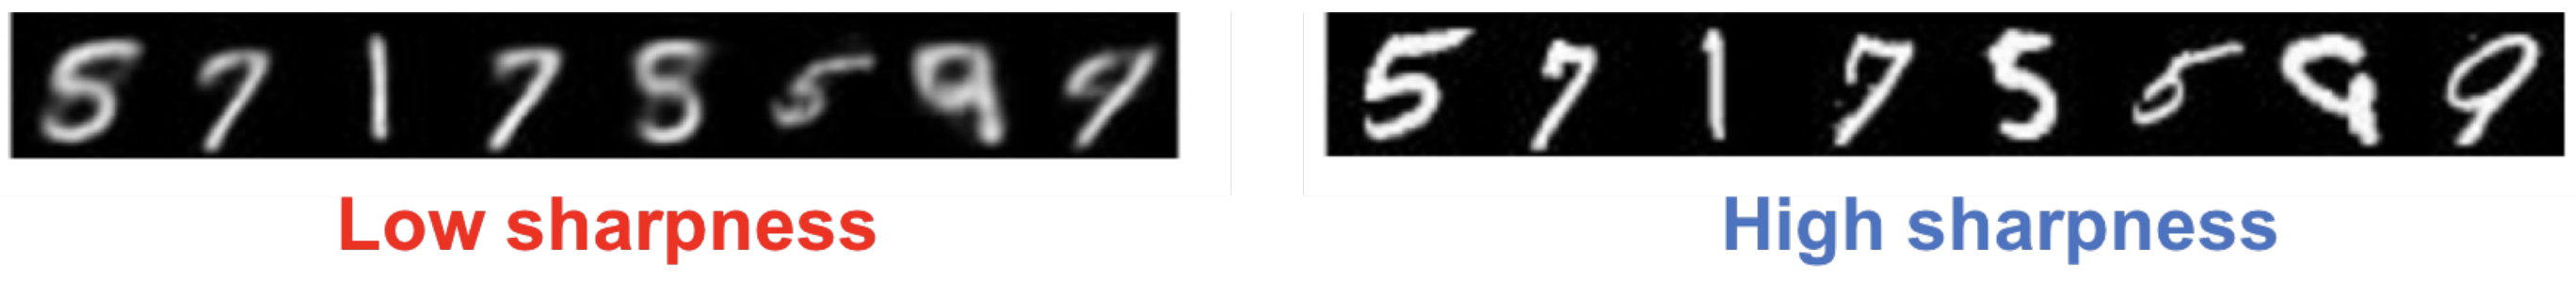
\includegraphics[width=0.9\linewidth]{figs/sharpness}
			\end{figure}
			$p(y | \bx)$ has low entropy (each image $\bx$ should have distinctly recognizable object).
			\item \textbf{Diversity}
			\begin{figure}
				\centering
				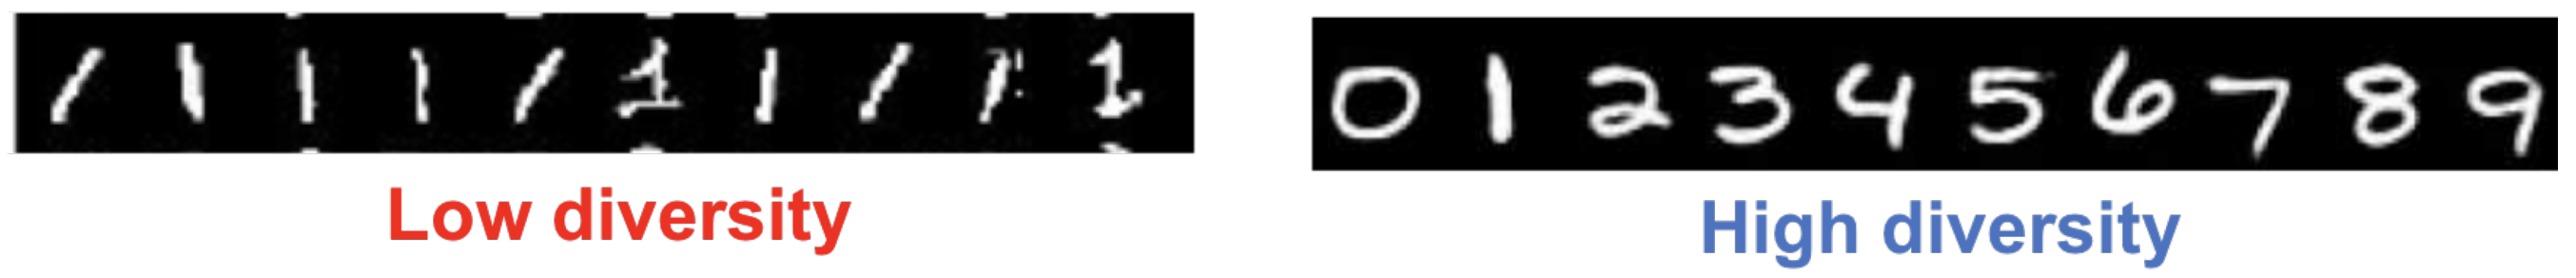
\includegraphics[width=0.9\linewidth]{figs/diversity}
			\end{figure}
			$p(y) = \int p(y | \bx) p(\bx) d \bx$ has high entropy (there should be as many classes generated as possible).
		\end{itemize}
	\end{block}
	\myfootnotewithlink{https://deepgenerativemodels.github.io}{image credit: https://deepgenerativemodels.github.io}
\end{frame}
%=======
\begin{frame}{Outline}
	\tableofcontents
\end{frame}
%=======
\section{Evaluation of likelihood-free models}
%=======
\subsection{Inception score}
%=======
\begin{frame}{Evaluation of likelihood-free models}
		\begin{block}{What do we want from samples?}
		\begin{itemize}
			\item Sharpness $\Rightarrow$ low $H(y | \bx) = - \sum_{y} \int_{\bx} p(y, \bx) \log p(y | \bx) d\bx$.
			\item Diversity $\Rightarrow$ high $H(y)  = - \sum_{y} p(y) \log p(y)$.
		\end{itemize}
	\end{block}
	\begin{block}{Inception Score}
		\vspace{-0.3cm}
		\footnotesize
		\begin{align*}
			IS &= \exp(H(y) - H(y | \bx)) \\ 
			&= \exp \left( - \sum_{y} p(y) \log p(y) + \sum_{y} \int_{\bx} p(y, \bx) \log p(y | \bx) d\bx\right) \\
			&= \exp \left( \sum_{y} \int_{\bx} p(y, \bx) \log \frac{p(y | \bx)}{p(y)} d\bx\right) \\ 
			&= \exp \left( \bbE_{\bx} \sum_{y} p(y | \bx) \log \frac{p(y | \bx)}{p(y)} \right) = \exp \left( \bbE_{\bx} KL(p(y | \bx) || p(y)) \right)
		\end{align*}
	\end{block}
	\myfootnotewithlink{https://arxiv.org/abs/1606.03498}{Salimans T. et al. Improved Techniques for Training GANs, 2016}
\end{frame}
%=======
\subsection{Frechet Inception Distance}
%=======
\begin{frame}{Evaluation of likelihood-free models}
	\begin{block}{Theorem (informal)}
		If $\pi(\bx)$ and $p(\bx | \btheta)$ has moment generation functions then
		\vspace{-0.1cm}
		\[
			\pi(\bx) = p(\bx | \btheta) \, \Leftrightarrow \, \bbE_{\pi} \bx^k = \bbE_{p} \bx^k, \quad \forall k \geq 1.
		\]
		\vspace{-0.7cm}
	\end{block}
	This is intractable to calculate all moments.
	\begin{block}{Frechet Inception Distance}
		\vspace{-0.3cm}
		\[
			FID (\pi, p) = \| \mathbf{m}_{\pi} - \mathbf{m}_{p}\|_2^2 + \text{Tr} \left( \bSigma_{\pi} + \bSigma_p - 2 \sqrt{\bSigma_{\pi} \bSigma_p} \right)
		\]
		\vspace{-0.5cm}
	\end{block}
	\begin{itemize}
		\item Representations are the outputs of the intermediate layer from the pretrained classification model.
		\item $\mathbf{m}_{\pi}$, $\bSigma_{\pi} $ are the mean vector and the covariance matrix of feature representations for samples from $\pi(\bx)$
		\item $\mathbf{m}_{p}$, $\bSigma_p$ are the mean vector and the covariance matrix of feature representations for samples from $p(\bx | \btheta)$.
	\end{itemize} 

	\myfootnotewithlink{https://arxiv.org/abs/1706.08500}{Heusel M. et al. GANs Trained by a Two Time-Scale Update Rule Converge to a Local Nash Equilibrium, 2017}
\end{frame}
%=======
\begin{frame}{Evaluation of likelihood-free models}
	\begin{figure}
		\centering
		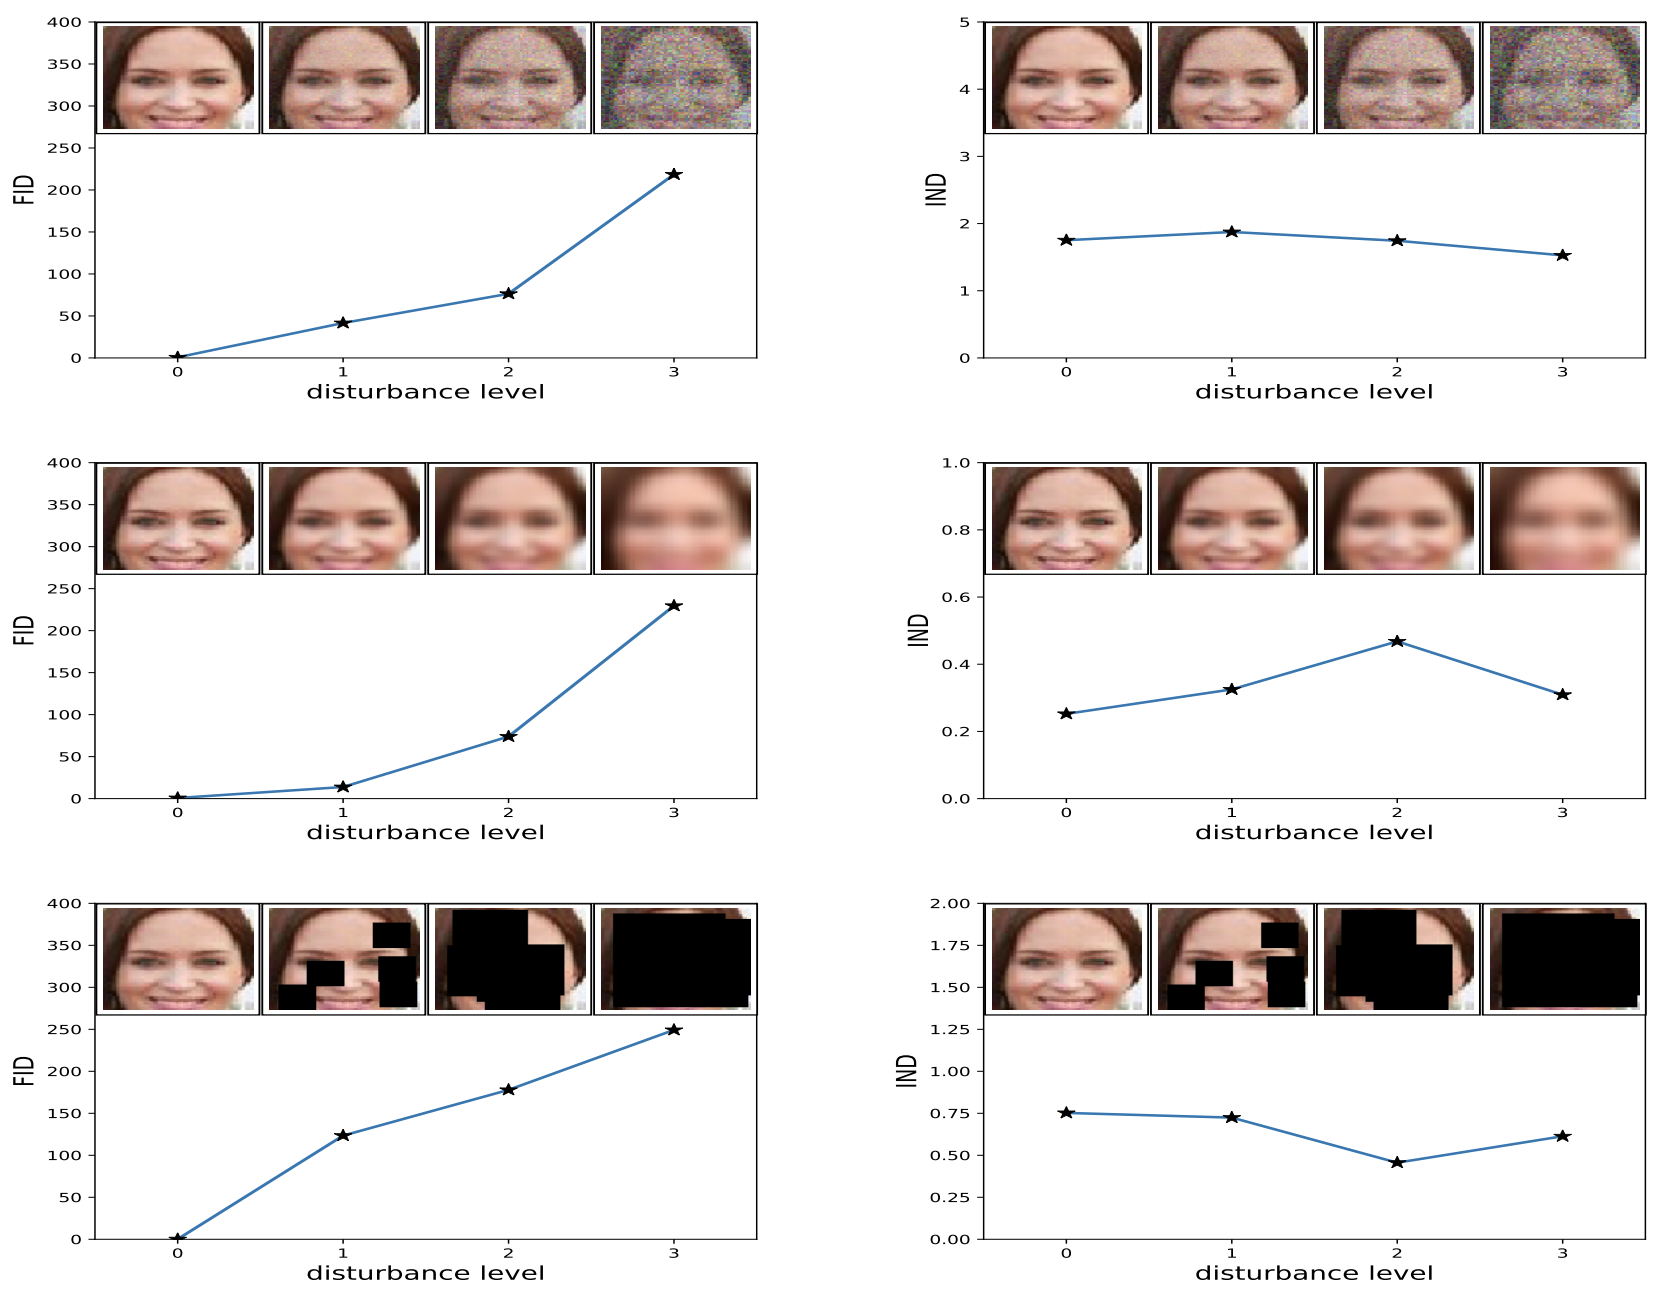
\includegraphics[width=0.9\linewidth]{figs/fid_results}
	\end{figure}
	
	\myfootnotewithlink{https://arxiv.org/abs/1706.08500}{Heusel M. et al. GANs Trained by a Two Time-Scale Update Rule Converge to a Local Nash Equilibrium, 2017}
\end{frame}
%=======
\begin{frame}{Limitations}
	\vspace{-0.5cm}
	\begin{block}{Inception Score}
		\vspace{-0.5cm}
		\[
			IS =  \exp \left( \bbE_{\bx} KL(p(y | \bx) || p(y)) \right)
		\]
		\vspace{-0.7cm}
	\end{block}
	\begin{itemize}
		\item If generator produces images with a different set of labels from the classifier training set, IS will be low.
		\item If generator produces one image per class, the IS will be perfect (there is no measure of intra-class diversity).
	\end{itemize}
	\begin{block}{Frechet Inception Distance}
		\vspace{-0.4cm}
		\[
			FID = \| \mathbf{m}_{\pi} - \mathbf{m}_{p}\|_2^2 + \text{Tr} \left( \bSigma_{\pi} + \bSigma_p - 2 \sqrt{\bSigma_{\pi} \bSigma_p} \right)
		\]
		\vspace{-0.7cm}
	\end{block}
	\begin{itemize}
		\item Needs a large sample size for evaluation.
		\item Calculation of FID is slow.
		\item Estimates only two sample moments.
	\end{itemize}
	Both scores depend on the pretrained classifier $p(y | \bx)$.

	\myfootnote{\href{https://arxiv.org/abs/1801.01973}{Barratt S., Sharma R. A Note on the Inception Score, 2018} \\
	\href{https://arxiv.org/abs/1706.08500}{Heusel M. et al. GANs Trained by a Two Time-Scale Update Rule Converge to a Local Nash Equilibrium, 2017}}
\end{frame}
%=======
\subsection{Precision-Recall}
%=======
\begin{frame}{Precision-Recall for Generative Models}
	\begin{block}{What do we want from samples}
		\begin{itemize}
			\item \textbf{Sharpness}: generated samples should be of high quality.
			\item \textbf{Diversity}: their variation should match that observed in the training set.
		\end{itemize}
	\end{block}
	\vspace{-0.5cm}
	\begin{figure}
		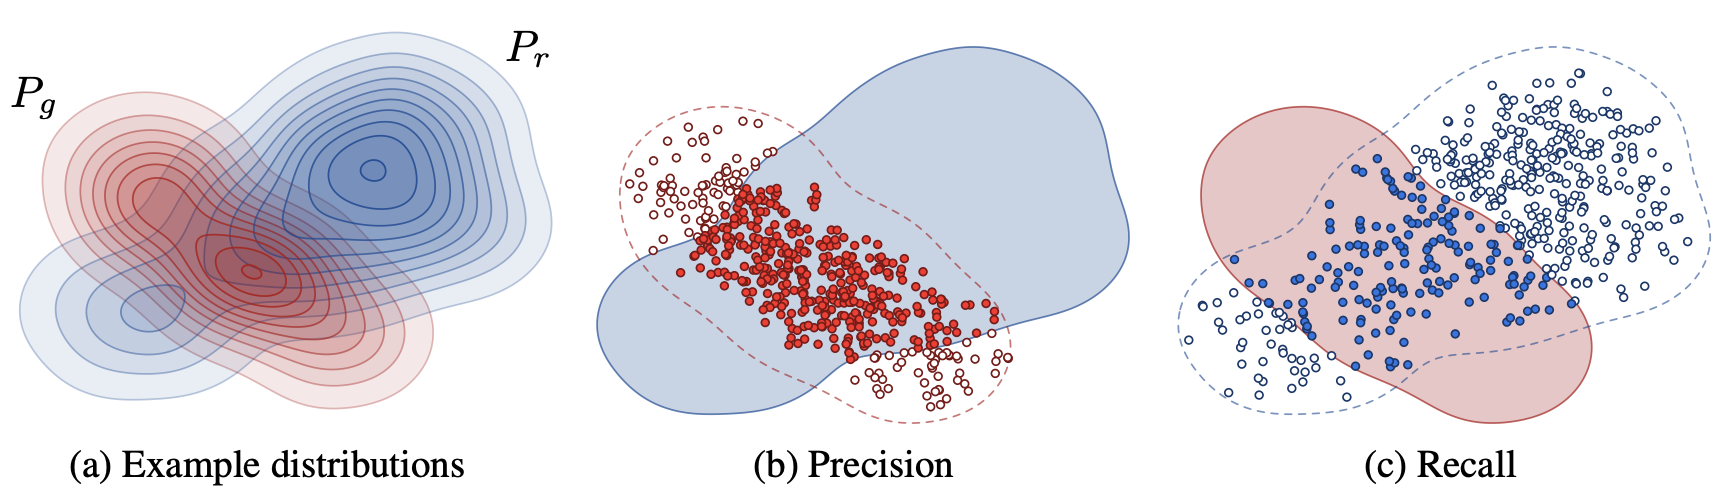
\includegraphics[width=0.95\linewidth]{figs/pr_curve}
	\end{figure}
	\vspace{-0.3cm}
	\begin{itemize}
		\item \textbf{Precision} denotes the fraction of generated images that are realistic.
		\item \textbf{Recall} measures the fraction of the training data manifold covered by the generator.
	\end{itemize}
	\myfootnotewithlink{https://arxiv.org/abs/1904.06991}{Kynkäänniemi T. et al. Improved precision and recall metric for assessing generative models, 2019}
\end{frame}
%=======
\begin{frame}{Precision-Recall for generative models}
	\begin{itemize}
		\item $\cS_{\pi} = \{\bx_i\}_{i=1}^{n} \sim \pi(\bx)$ -- real samples;
		\item $\cS_{p} = \{\bx_i\}_{i=1}^{n} \sim p(\bx | \btheta)$ -- generated samples.
	\end{itemize}
	Embed samples using pretrained classifier network (as previously):
	\[
		\cG_{\pi} = \{\mathbf{g}_i\}_{i=1}^n, \quad \cG_{p} = \{\mathbf{g}_i\}_{i=1}^n.
	\]
	Define binary function:
	\[
		f(\mathbf{g}, \cG) = 
		\begin{cases}
			1, \quad \text{if exists } \mathbf{g}' \in \cG: \| \mathbf{g}  - \mathbf{g}'\|_2 \leq \| \mathbf{g}' - \text{NN}_k(\mathbf{g}', \cG)\|_2; \\
			0, \quad \text{otherwise.}
		\end{cases}
	\]
	\[
		\text{Precision} (\cG_{\pi}, \cG_{p}) = \frac{1}{n} \sum_{\mathbf{g} \in \cG_{p}} f(\mathbf{g}, \cG_{\pi}); \,\, \text{Recall} (\cG_{\pi}, \cG_{p}) = \frac{1}{n} \sum_{\mathbf{g} \in \cG_{\pi}} f(\mathbf{g}, \cG_{p}).
	\]
	\vspace{-0.4cm}
	\begin{figure}
		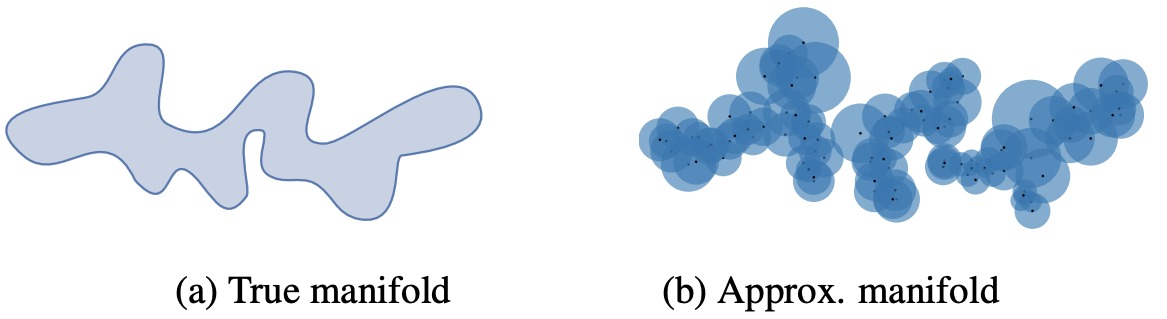
\includegraphics[width=0.7\linewidth]{figs/pr_k_nearest}
	\end{figure}
	\myfootnotewithlink{https://arxiv.org/abs/1904.06991}{Kynkäänniemi T. et al. Improved precision and recall metric for assessing generative models, 2019}
\end{frame}
%=======
\begin{frame}{Precision-Recall for generative models}
	\begin{figure}
		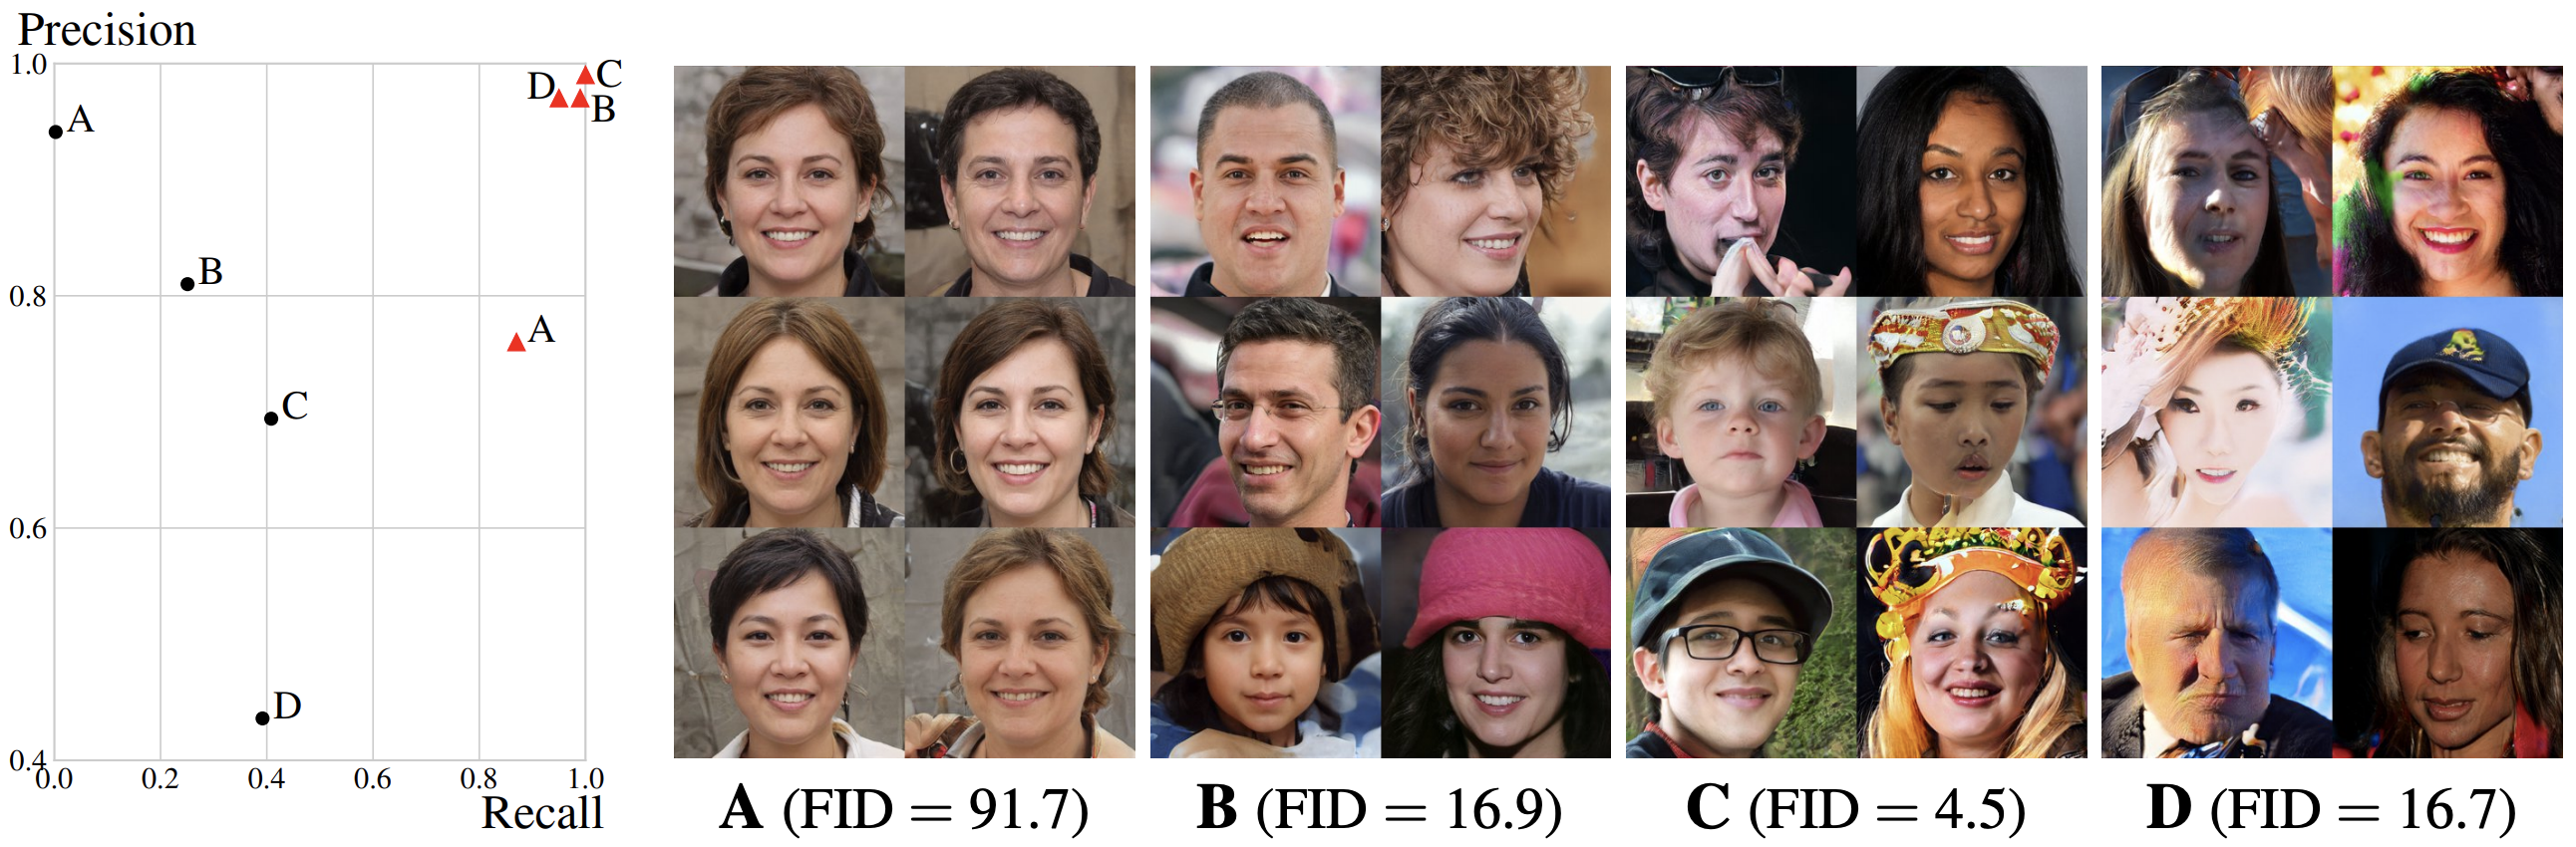
\includegraphics[width=\linewidth]{figs/pr_vs_fid}
	\end{figure}
	\begin{figure}
		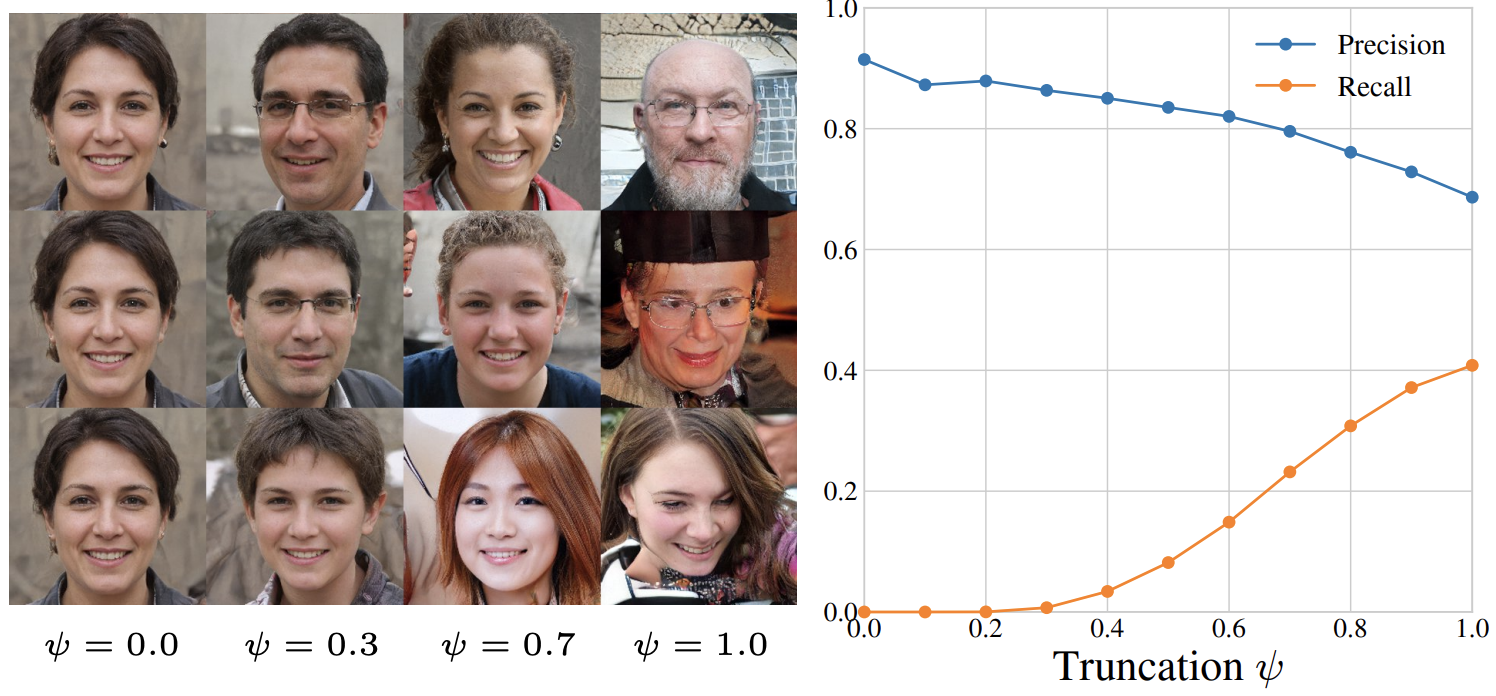
\includegraphics[width=0.75\linewidth]{figs/pr_truncation}
	\end{figure}
	\myfootnotewithlink{https://arxiv.org/abs/1904.06991}{Kynkäänniemi T. et al. Improved precision and recall metric for assessing generative models, 2019}
\end{frame}
%=======
\begin{frame}{Truncation trick}
	\begin{block}{BigGAN: truncated normal sampling}
		\vspace{-0.3cm}
		\[
			p(\bz | \psi) = \cN(\bz | 0, 1) / \int_{-\infty}^\psi \cN(\bz | 0, 1) d\bz
		\]
		Components of $\bz \sim \cN(0, \bI)$ which fall outside a predefined range are resampled.
	\end{block}
	
	\begin{block}{StyleGAN}
		\vspace{-0.2cm}
		\[
			\bz' = \hat{\bz} + \psi \cdot (\bz - \hat{\bz}), \quad \hat{\bz} = \bbE_{\bz} \bz
		\]
		\vspace{-0.2cm}
		\begin{itemize}
			\item Constant $\psi$ is a tradeoff between diversity and fidelity. 
			\item $\psi=0.7$ is used for most of the results.
		\end{itemize}
	\end{block}

	\myfootnote{\href{https://arxiv.org/abs/1809.11096}{Brock A., Donahue J., Simonyan K. Large Scale GAN Training for High Fidelity Natural Image Synthesis, 2018} \\
	\href{https://arxiv.org/abs/1812.04948}{Karras T., Laine S., Aila T. A Style-Based Generator Architecture for Generative Adversarial Networks, 2018}}
\end{frame}
%=======
\section{Discrete VAE latent representations}
%=======
\begin{frame}{Discrete VAE latents}
	\begin{block}{Motivation}
		\begin{itemize}
			\item Previous VAE models had \textbf{continuous} latent variables $\bz$.
			\item \textbf{Discrete} representations $\bz$ are potentially a more natural fit for many of the modalities.
			\item Powerful autoregressive models (like PixelCNN) have been developed for modelling distributions over discrete variables.
			\item All cool transformer-like models work with discrete tokens.
		\end{itemize}
	\end{block}
	\begin{block}{ELBO}
		\vspace{-0.3cm}
		\[
		\mathcal{L} (\bphi, \btheta)  = \mathbb{E}_{q(\bz | \bx, \bphi)} \log p(\bx | \bz , \btheta) - KL(q(\bz| \bx, \bphi) || p(\bz)) \rightarrow \max_{\bphi, \btheta}.
		\]
		\vspace{-0.5cm}
	\end{block}
	\begin{itemize}
		\item Reparametrization trick to get unbiased gradients.
		\item Normal assumptions for $q(\bz | \bx, \bphi)$ and $p(\bz)$ to compute KL analytically.
	\end{itemize}
\end{frame}
%=======
\begin{frame}{Discrete VAE latents}
	\begin{block}{Assumptions}
		\begin{itemize}
			\item Define dictionary (word book) space $\{\be_k\}_{k=1}^K$, where $\be_k \in \bbR^C$, $K$ is the size of the dictionary.
			\item Let $c \sim \text{Categorical}(\bpi)$, where 
			\vspace{-0.6cm}
			\[
			\bpi = (\pi_1, \dots, \pi_K), \quad \pi_k = P(c = k), \quad \sum_{k=1}^K \pi_k = 1.
			\]
			\vspace{-0.6cm}
			\item Let VAE model has discrete latent representation $c$ with prior $p(c) = \text{Uniform}\{1, \dots, K\}$.
		\end{itemize}
	\end{block}
	\vspace{-0.3cm}
	\begin{block}{How it should work?}
		\begin{itemize}
			\item Our variational posterior $q(c | \bx, \bphi) = \text{Categorical}(\bpi(\bx, \bphi))$ (encoder) outputs discrete probabilities vector.
			\item We sample $c^*$ from $q(c | \bx, \bphi)$ (reparametrization trick analogue).
			\item Our generative distribution $p(\bx | \be_{c^*}, \btheta)$ (decoder).
		\end{itemize}
	\end{block}
\end{frame}
%=======
\begin{frame}{Discrete VAE latents}
	\begin{block}{ELBO}
		\vspace{-0.5cm}
		\[
		\mathcal{L} (\bphi, \btheta)  = \mathbb{E}_{q(c | \bx, \bphi)} \log p(\bx | c, \btheta) - KL(q(c| \bx, \bphi) || p(c)) \rightarrow \max_{\bphi, \btheta}.
		\]
		\vspace{-0.5cm}
	\end{block}
	\begin{block}{KL term}
		\vspace{-0.8cm}
		\begin{multline*}
			KL(q(c| \bx, \bphi) || p(c)) = \sum_{k=1}^K q(k | \bx, \bphi) \log \frac{q(k | \bx, \bphi)}{p(k)} = 
			\\ = \color{violet}{\sum_{k=1}^K q(k | \bx, \bphi) \log q(k | \bx, \bphi)}  \color{teal}{- \sum_{k=1}^K q(k | \bx, \bphi) \log p(k)}  = \\ = \color{violet}{- H(q(c | \bx, \bphi))} + \color{teal}{\log K}. 
		\end{multline*}
		\vspace{-0.6cm}
	\end{block}
	\begin{itemize}
		\item Is it possible to make reparametrization trick? (we sample from discrete distribution now!).
		\item Entropy term should be estimated.
	\end{itemize}
\end{frame}
%=======
\begin{frame}{Summary}
	\begin{itemize}
		\item Inception Score and Frechet Inception Distance are the common metrics for GAN evaluation, but both of them have drawbacks.
		\vfill
		\item Precision-recall allows to select model that compromises the sample quality and the sample diversity.	
		\vfill 
		\item Truncation tricks help to select model with compomised samples: diverse and sharp.
		\vfill
		\item Discrete VAE latents is a natural idea, but we have to avoid non-differentiable sampling operation.
	\end{itemize}
\end{frame}
\end{document} 